
\documentclass[journal]{IEEEtran}
\usepackage{tikz}
\usetikzlibrary{decorations.pathreplacing,angles,quotes}

% correct bad hyphenation here
\hyphenation{op-tical net-works semi-conduc-tor}

\begin{document}
%
% paper title
\title{Paper Discussion Report}

% puts info about authors at bottom of first page
\author{Lawrence~Owusu,~Jordan~Sturtz,~and~Swetha~Chittam~% <-this % stops a space
  \thanks{The authors are graduate students at NCA\&T}% <-this % stops a space
}

% note the % following the last \IEEEmembership and also \thanks -
% these prevent an unwanted space from occurring between the last author name
% and the end of the author line. i.e., if you had this:
%
% \author{....lastname \thanks{...} \thanks{...} }
%                     ^------------^------------^----Do not want these spaces!

% The paper headers
% The only time the second header will appear is for the odd numbered pages
% after the title page when using the twoside option.
\markboth{CS851 - Deep Learning: Paper Discussion Report}%
{Shell \MakeLowercase{\textit{et al.}}: CS851 - Deep Learning: Method Discussion Report}

% make the title area
\maketitle

% As a general rule, do not put math, special symbols or citations
% in the abstract or keywords.
% \begin{abstract}
% The abstract goes here.
% \end{abstract}

% Note that keywords are not normally used for peerreview papers.
% \begin{IEEEkeywords}
% IEEE, IEEEtran, journal, \LaTeX, paper, template.
% \end{IEEEkeywords}

% For peer review papers, you can put extra information on the cover
% page as needed:
% \ifCLASSOPTIONpeerreview
% \begin{center} \bfseries EDICS Category: 3-BBND \end{center}
% \fi

%
% For peerreview papers, this IEEEtran command inserts a page break and
% creates the second title. It will be ignored for other modes.
\IEEEpeerreviewmaketitle

\section{Summary}

  %
  % Here we have the typical use of a "T" for an initial drop letter
  % and "HIS" in caps to complete the first word.
  \IEEEPARstart{A}{} paper authored by Gunasekaran, et al. uses deep learning methods
  to classify viruses by their DNA sequences[1]. Since DNA is composed of strings
  of nucleotides, the problem amounts to classifying viruses according to samples of nucleotide
  strings. The authors collect data from the public nucleotide sequence database,
  The National Centre for Biotechnology Information (NCBI) https://www.ncbi.nlm.nih.gov.
  They then encode this data using label encoding and k-mer encoding. For each encoding type,
  they run three different deep learning models: CNN, CNN-LSTM, and CNN-Bidirectional-LSTM.
  The architectures of all three models start with embedding layers, then convolutional layers,
  then max pooling layers, and then from there diverge to either add LSTM layers or
  bidirectional LSTM layers before finishing with dense layers and a final output layer.
  The authors compare all six combinations of the two encoding methods with the three model types
  using several performance metrics. They also compare their results to current state-of-the-art
  approaches in the literature.

\section{Problem Statement}
  All DNA and RNA is composed of a string of nucleotides. A nucleotide refers to one of
  four compounds for DNA (adenine, cytocine, guanine, thymine) or four compounds for RNA
  (adenine, cytocine, guanine, uracil). For double-helix DNA or RNA, each nucleotide
  bonds with one and only one other nucleotide, forming what is called a base pair (Fig 1). Since
  these base pairs are fixed, then, a DNA or RNA sequence can be identified solely by one
  side of the double helix. Thus, every DNA virus can be identified by a single string of
  characters drawn from the set $\{A, C, G, T\}$ and every RNA virus can be identified by a string
  of characters drawn from the set $\{A, C, G, U\}$. The task, then, is to build highly accurate
  models to classify a virus from its DNA or RNA sample.

  \begin{figure}
    \centering
    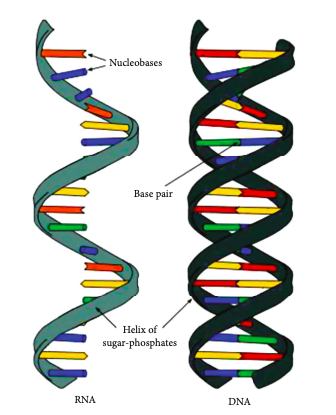
\includegraphics[width=8cm]{figures/dna.png}
    \caption{Single or double-stranded DNA/RNA, borrowed from Gunasekaran, H., et al.[1]}
  \end{figure}

\section{Related Work}
  DNA classification and protein structure-sequence prediction remain some of the challenges in the field of computational biology.
  Determination of accurate protein structure and DNA sequence are important in developing deep understanding of the functions of protein,
  disease diagnosis, prevention of epidemics and assisting in drug design [2].
  \subsection{Non-Machine Learning Methods}

    Although experimental methods of protein structure determination, including Cryogenic Electron Microscopy,
    X-ray Crystallography, Nuclear Magnetic Resonance Spectroscopy and others have seen continuous advancement,
    such techniques are expensive, involve cumbersome and time-consuming procedures and require high level expertise.
    Similarly, DNA-based approaches such as DNA sequencing, DNA-DNA hybridization and DNA fingerprinting for the identification
    and classification of species of bacteria and viruses have some challenges. For example, these DNA sequencing technologies
    produce read length as short as 35-40 nucleotides, thus posing challenges for genome annotation and assembly [3].
    To make the process less cumbersome, deep learning algorithms as well as hybrid deep learning models have been proposed
    for DNA and protein sequence classification [4].

  \subsection{Machine Learning Methods}
    The use of CNN and LSTM models in protein sequence prediction, classification of miRNA and DNA sequence classification is
    highly researched in computational biology. Abdulkadir and Baha (2021) applied a hybrid deep learning model based on
    CNN and LSTM to classify miRNA with accuracy, sensitivity, specificity and F1 scores of 0.943, 0.935, 0.948 and 0.925 respectively,
    suggesting that the hybrid CNN and LSTM networks can be employed to achieve better performance for pre-miRNA classification [5].
    Similarly, Chinju and his colleagues (2022) developed a hybrid deep learning CNN-LSTM model that uses the
    convolutional neural network architecture and long short-term memory network to classify the protein sequences belonging to
    the five-member polo like kinase family with an accuracy score of 97.6\% [6].
    LSTM networks have been used tremendously in computational biology especially in protein structure prediction.
    For example, Soren and Winther (2019) reported 67.4\% performance accuracy on protein structure prediction problems [7].

\subsection{Model Performance Against State of the Art Methods}

  The authors compare their accuracy results to other state-of-the-art approaches to
  virus classification (Fig 2). Their results show that all three of their models show higher accuracy than
  that achieved by Nguyen, et al.[8], Do, et al.[9], and Zhang, et al.[10].

  \begin{figure}
    \centering
    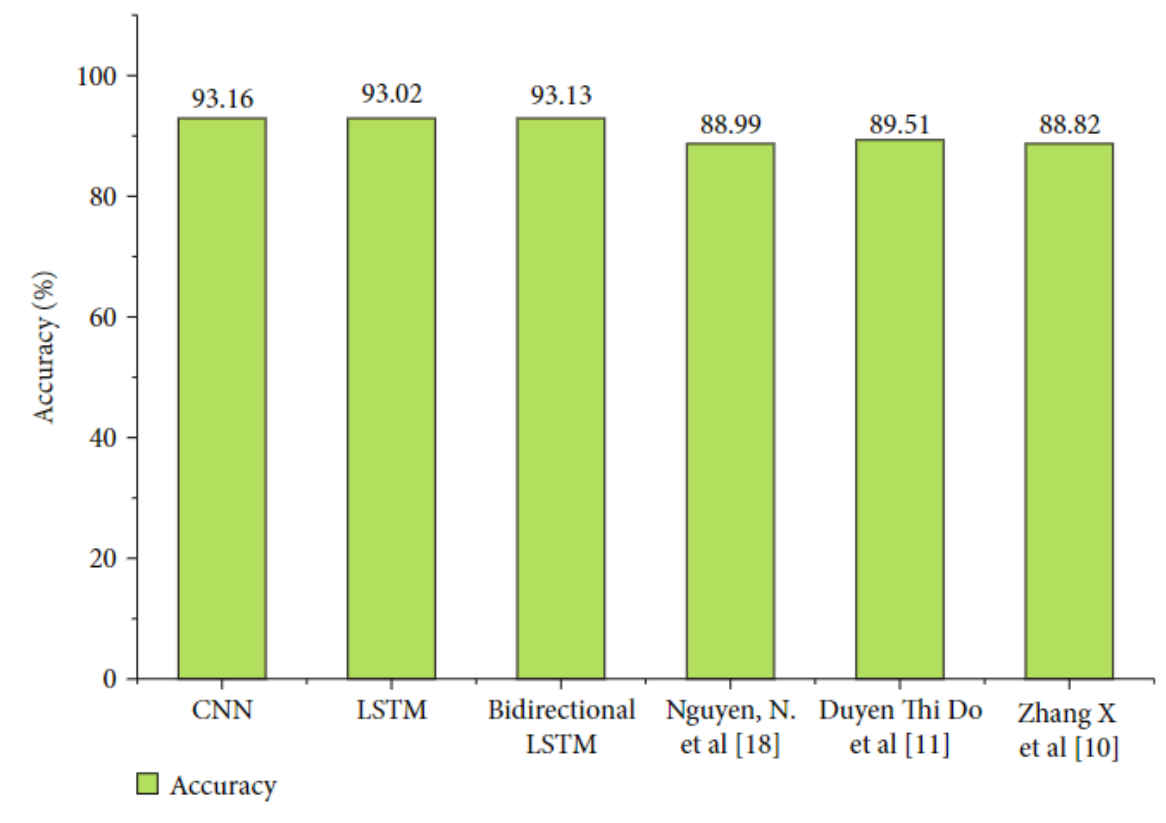
\includegraphics[width=8cm]{figures/accuracy_compared_to_state_of_art.png}
    \caption{Gunasekaran, H. et al, compared against state of the art methods, borrowed from Gunasekaran, et al. (2020)}
  \end{figure}

\section{Data Collection}
  The authors obtain complete genomic sequences from the
  National Centre for Biotechnology Information (NCBI) https://www.ncbi.nlm.nih.gov/.
  Sequence length ranges from 8 to 37971 nucleoids. They collected genomic sequences
  for six virus classes: COVID, MERS, SARS, Dengue, Hepatitus, and Influenza (Fig 3).
  Because the population of these viruses were unbalanced--for instance, there were 37272
  samples of COVID and only 1418 samples of MERS--the authors opted to use
  Synthetic Minority Oversampling Technique (SMOTE) to get a more even distribution of
  all six classes in their dataset.
  The DNA sequence dataset used in this paper consists of 66,153 inputs which is divided into training,
  validation and testing sets with a ratio of 70\%, 10\% and 20\% respectively.
  The training set consists of 46307, and the validation set consists of 6615, and the testing set consists of 13231 samples.
  The maximum sequence length is 2000, and the vocabulary size is 8972.

  \begin{figure}
    \centering
    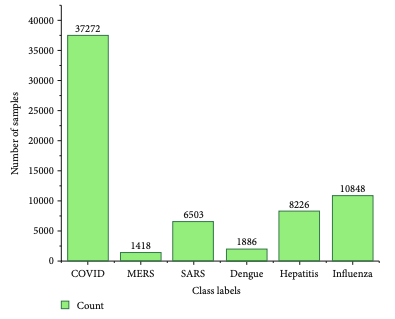
\includegraphics[width=8cm]{figures/data_collection.png}
    \caption{Samples of virus classes retrieved from NCBI, borrowed from Gunasekaran, H., et al. (2020)}
  \end{figure}

\section{Data Preprocessing}
  The authors encoded the data in two different formats for comparative analysis.
  In the first approach, they use label encoding, which replaces each nucleoid by a unique index value,
  preserving positional information (Fig 4).
  In the second approach, they used k-mer encoding, which generates all k-mers from a sequence
  and forms an English-like sentence onto which natural language processing techniques
  can be applied (Fig 5).

  \begin{figure}
    \centering
    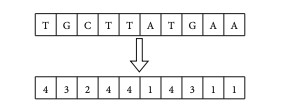
\includegraphics[width=8cm]{figures/label_encoding.png}
    \caption{Label encoding example, borrowed from Gunasekaran, H., et al. (2020)}
  \end{figure}

  \begin{figure}
    \centering
    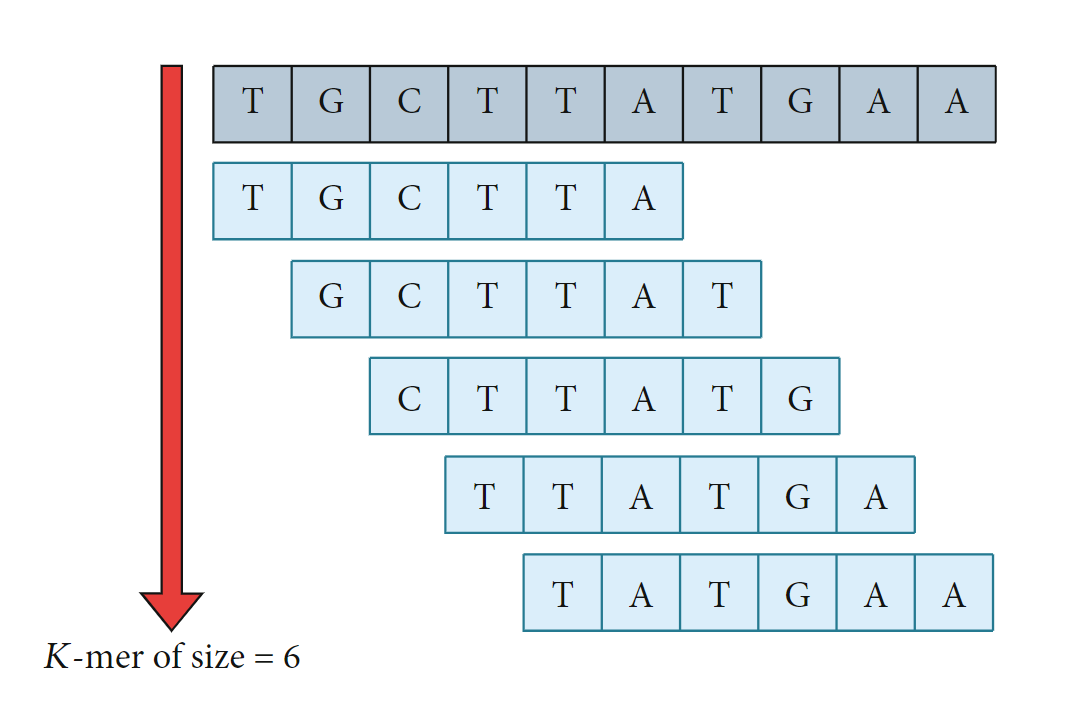
\includegraphics[width=8cm]{figures/kmer_encoding.png}
    \caption{K-mer encoding example, where k=6, borrowed from Gunasekaran, H., et al. (2020)}
  \end{figure}

  Once encoded, in both cases the input data is one-hot encoded and then fed into
  the first layer of the models, which is an embedding layer.

\section{Proposed Models}
  In this paper, the authors use three different classification models to perform multi-classification
  of the DNA sequence: CNN, CNN-LSTM and CNN-bidirectional LSTM.
  All three models share the same initial layers: an embedding layer, convolutional layers, and
  max pooling layers. The raw data is first either label encoded or k-mer encoded and then
  one-hot encoded to be fed into the embedding layer. The results of the embedding layer
  are then fed into the convolutional layers, each of which has a corresponding max pooling layer.
  From here, the three model types diverge. For the CNN model, the results are fed into
  the final dense layers and output layers. The LSTM and bidirectional LSTM models differ only
  in that they add LSTM or bidirectional LSTM respectively before the final dense layers.

  \subsection{CNN}
    CNN is a popular deep learning technique that is widely used for feature extraction
    and to solve any classification problems.
    CNN can be used for any kind of datasets like text, image, or video datasets.
    The 2D CNN is often used for feature extraction from image datasets and
    3D CNN is used for feature extraction from video datasets.
    The 1D CNN auto extracts the features from the input dataset and can therefore be used
    for text classification. Here in this paper, authors are using 1D CNN for feature extraction
    of the DNA sequence data. The proposed CNN model architecture has two 1D convolutional layers,
    each followed by a max pooling layer to reduce the feature map dimensions from the previous layers.
    Next, a flatten layer is used to convert feature maps to a single column vector followed by multiple dense layers.
    The output is passed to the final dense layer with softmax activation function to perform multi-classification.

    Table I shows the hyper parameters for the proposed CNN model.
    \begin{table}
      \caption{\label{tab:table-name}Hyper parameters of CNN model}
      \centering
      \resizebox{\columnwidth}{!}{%
        \begin{tabular}{ || l l l l l l l ||}
        \hline
        Layers           & Units & Filters & Kernel & Act. Func & Output Shape & Params   \\
        \hline
        \hline
        Embedding        & 8     &         &        &           & (None, 1000, 8)   & 128   \\
        Conv 1D          &       & 128     & 2*2    & ReLu      & (None, 1000, 128) & 3200  \\
        Max Pool         &       &         & 2*2    &           & (None, 500, 128)  & 0     \\
        Conv 1D          &       & 64      & 2*2    & ReLu      & (None, 500, 64)   & 24640 \\
        Max Pool         &       &         & 2*2    &           & (None, 250, 64)   & 0     \\
        Flatten          &       &         &        &           & (None, 16)        & 0     \\
        Dense            & 128   &         &        &           & (None, 128)       & 2176  \\
        Dense            & 64    &         &        &           & (None, 64)        & 8256  \\
        Dense            & 6     &         &        & Softmax   & (None, 6)         & 390   \\
        \hline
        \end{tabular}%
      }
    \end{table}

  \subsection{CNN-LSTM}
    Long-short term memory (LSTM) is a recurrent neural network that can learn long term dependencies in a sequence and
    hence can be used for sequence classification or prediction. The LSTM model consists of three gates: forget gate, input gate and output gate (Fig 6).
    For the hybrid CNN-LSTM model, the authors add an LSTM Layer with 100 LSTM memory units
    between the final convolutional layer and the final dense layers.

    \begin{figure}
      \centering
      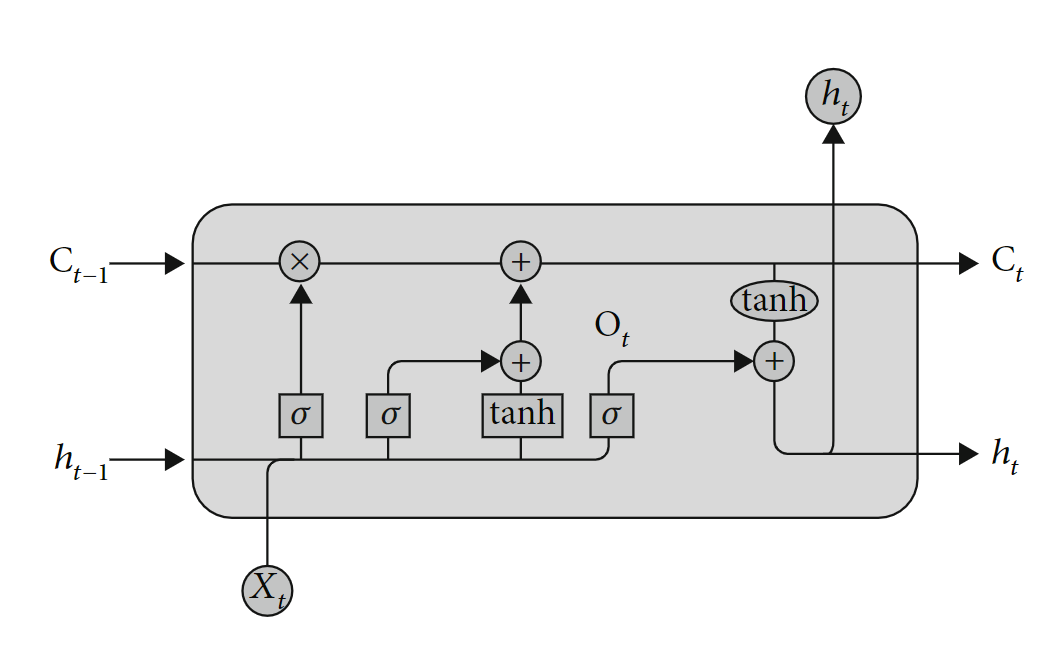
\includegraphics[width=8cm]{figures/lstm_cell.png}
      \caption{LSTM Cell Architecture. x is a multiplicative gate, + is additive, borrowed from Gunasekaran, H., et al. (2020)}
    \end{figure}


    % I think this explanation could be better. Also might not need to be included
    % The current state is a function of both the previous hidden state and the
    % current input: $h(t) = f(h(t-1), x(t))$.
    % The forget gate is responsible for removing any information from the cell state.
    % When the information becomes invalid, it outputs zero.
    % The input gate is responsible for adding relevant information to the cell state,
    % this gate uses two activation functions sigmoid and tanh.
    % The output gate is responsible to output the current cell state h(t) by employing sigmoid and tanh
    % activation functions.

  \subsection{CNN-Bidirectional-LSTM}
    The bi-directional LSTM has two RNN’s: One to learn dependencies in forward direction and the other to
    learn dependencies in backward direction (Fig 7). For the hybrid CNN-LSTM-Bidirectional model, the authors add the bidirectional LSTM layers
    after the final convolutional layers and before the final dense layers.

    \begin{figure}
      \centering
      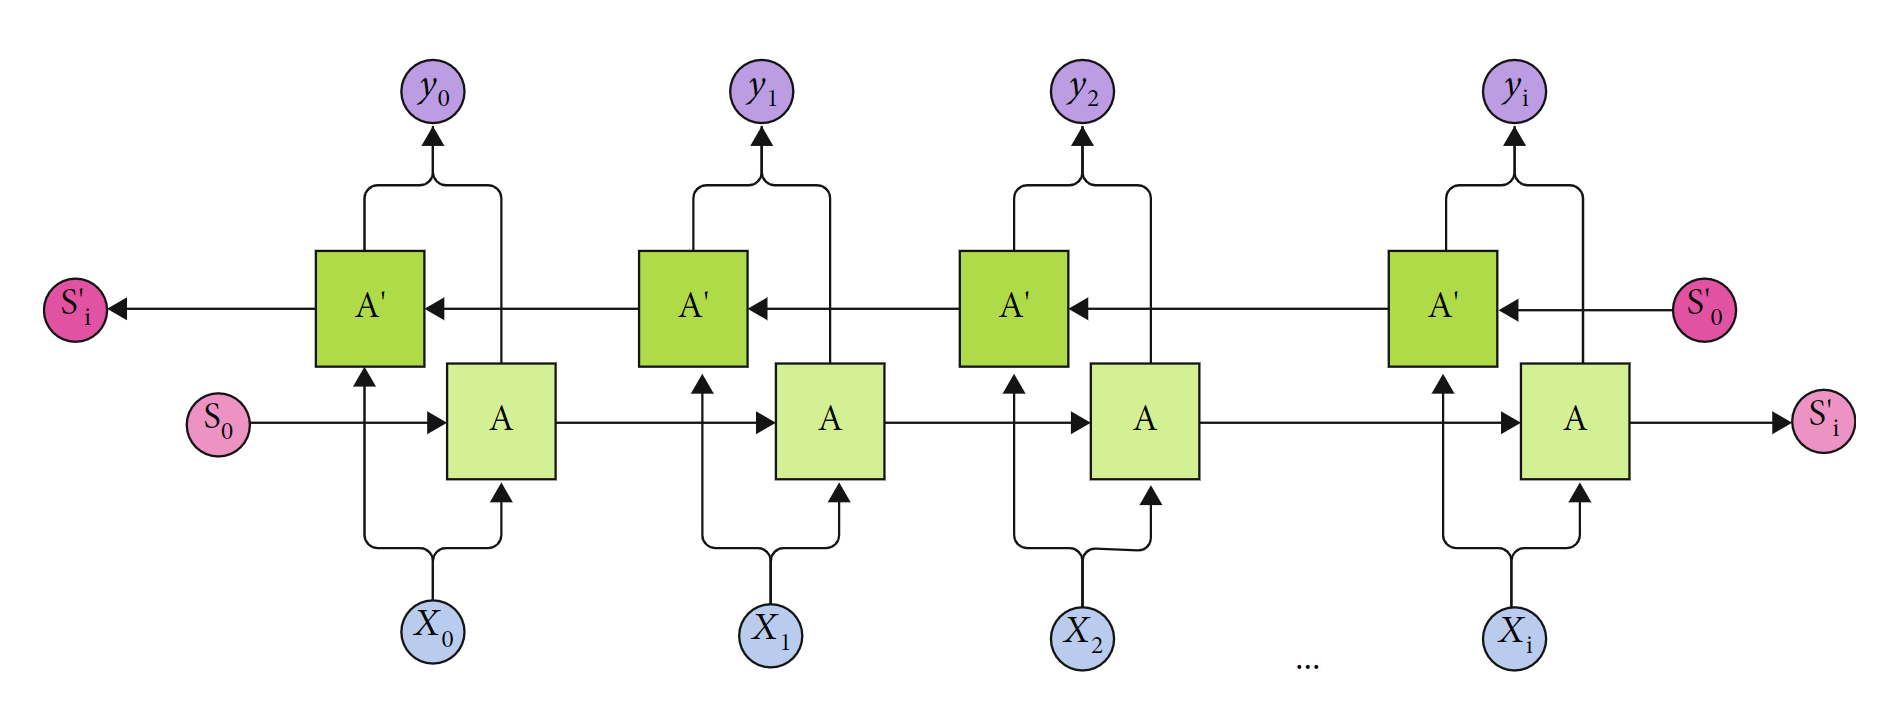
\includegraphics[width=8cm]{figures/bi_lstm_cell.png}
      \caption{Bidirectional LSTM Model Architecture, borrowed from Gunasekaran, et al. (2020)}
    \end{figure}

\section{Results and Discussion}
  The proposed models CNN, CNN-LSTM, CNN-Bi-LSTM models are tested by varying different hyperparameters listed in Table I.
  The authors use the grid-search cross-validation technique to find the best parameters of the model.
  The best parameters are listed in Table II.

  \begin{table}
    \caption{\label{tab:table2}Best Hyperparameters}
    \centering
    % \resizebox{\columnwidth}{!}{%
      \begin{tabular}{ || l l ||}
      \hline
      Parameters & Values \\
      \hline
      \hline
      Size of Filter       & 2*2 \\
      Training Batch Size  & 100 \\
      Training Epochs      & 10  \\
      Embedding Dimensions & 32  \\
      K-mer Size           & 6   \\
      \hline
      \end{tabular}%
    % }
  \end{table}

  The classification models are evaluated using different classification metrics like accuracy, precision, recall, F1 score, sensitivity,
  and specificity by obtaining the confusion matrix for both k-mer and label encoding techniques.
  The confusion matrix holds the values of true positives (TP), true negatives (TN), false positives (FP), and false negatives (FN).
  Based on these values, classification metrics are calculated and compared.
  Table III shows the formulas for calculating these classification metrics.
  \begin{table}
    \caption{\label{tab:table3}Formulas to Calculate Performance Metrics}
    \centering
    % \resizebox{\columnwidth}{!}{%
      \begin{tabular}{ || l l ||}
      \hline
      Metric & Formula \\
      \hline
      \hline
      Accuracy    & $\frac{TP + TN}{TP + TN + FP + FN}$\\
      Specificity & $\frac{TN}{TN + FP}$ \\
      Sensitivity & $\frac{TP}{TP + FN}$ \\
      Precision   & $\frac{TP}{TP + FP}$ \\
      \hline
      \end{tabular}%
    % }
  \end{table}

  \subsection{Model Comparison}
    Figure 8 shows the accuracy comparison for all three models for training and testing data using label and k-mer encoding.
    The testing accuracies for label encoding are less when compared to its training accuracy.
    For k-mer encoding testing accuracies are more significant than training.
    Therefore, the encoding technique plays an important role for achieving high accuracy.

    \begin{figure}
      \centering
      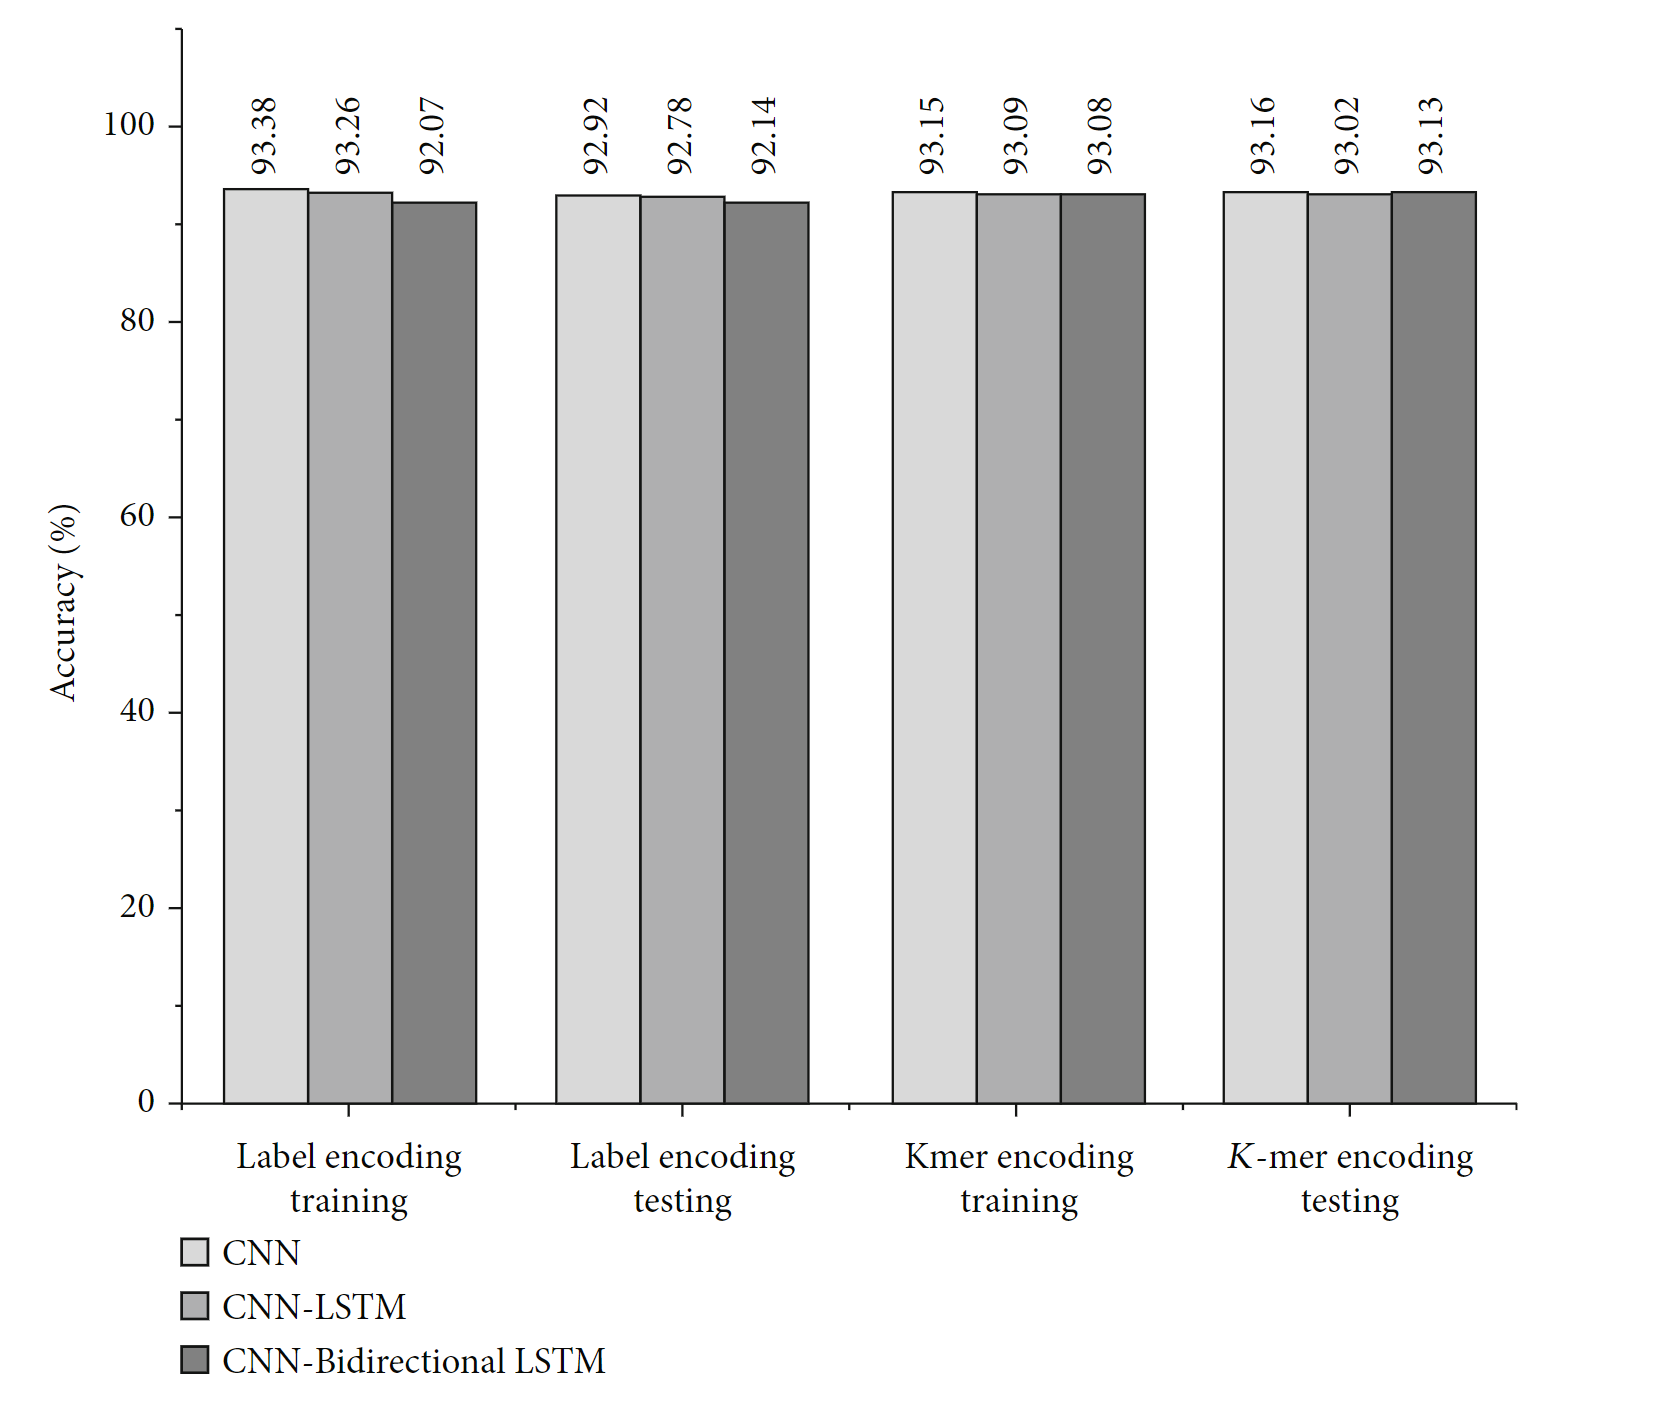
\includegraphics[width=8cm]{figures/accuracy.png}
      \caption{Training and Testing Accuracies of all six models, borrowed from Gunasekaran, et al. (2020)}
    \end{figure}

    Figure 9 shows the training and validation accuracies for all three models and both encodings.
    From Figure 9, we can observe that the accuracy of the model remains same after 10 epochs for all models
    except CNN-LSTM using k-mer encoding. This model has unstable accuracy as each epoch increases.
    CNN and CNN-Bi-LSTM have high accuracies of 93.16\%, 93.13\% respectively, when compared to LSTM.

    \subsection{Discussion}
      Figure 10 shows the model performance  concerning six different classes using label and k-mer encoding techniques.
      Based on metrics in Figure 10, we make the following observations:
      \begin{itemize}
        \item If class samples are high, CNN with label encoding has high precision.
        \item If class samples are low, CNN with k-mer encoding has high precision.
        \item If recall is preferred, k-mer encoding has higher recall for all classes irrespective of the class samples.
        \item High sensitivity rate of 99.95\% is obtained for class “a” using CNN+Bi-LSTM with label encoding.
        \item To obtain a high recall and sensitivity for class with more samples, Bi-LSTM with label encoding will be a good choice.
        \item CNN with label encoding offers high specificity irrespective of the class size.
      \end{itemize}
      CNN with label encoding outperforms other two models but their testing accuracies are low.
      K-mer encoding has achieved high validation and testing accuracy.
      We can conclude that, the best model can be chose not only based on the accuracy of the model
      but also other metrics such as sensitivity, specificity and precision must be considered.

\section{Conclusion}
  The authors' results are promising when compared to existing non machine-learning and machine learning methods for
  virus classification. The various performance metrics reviewed here show that the right model may depend on the
  particular use case. If accuracy is the most important metric, then the authors' results show that CNN outperforms
  CNN-LSTM and CNN-bidrectional LSTM. The high accuracy acheived in this paper demonstrates the effectiveness of
  deep learning models in performing complex tasks.

\begin{thebibliography}{1}

\bibitem{IEEEhowto:kopka}
  H.~Gunasekaran, K.~Ramalakshmi, A.~Rex~Macedo~Arokiaraj, S.~Deepa~Kanmani, C.~Venkatesan, and C.~Suresh~Gnana~Dhas.
  "Analysis of DNA Sequence Classification Using CNN and Hybrid Models."
  \emph{Computational and mathematical methods in medicine}, 2021.
\bibitem{IEEEhowto:kopka}
  S.~Shadab,~M.~T.~Alam~Khan,~N.~A.~Neezi,~S.~Adilina,~and~S.~Shatabda,
  “DeepDBP: deep neural networks for identification of DNA-binding proteins,”
  \emph{Informatics in Medicine Unlocked}, vol. 19, article 100318, 2020.
\bibitem{IEEEhowto:kopka}
  M~.Pop and S~Salzberg. "Bioinformatics challenges of new sequencing technology."
  \emph{Trends Genet}. vol. 24, no. 3, 142-149. 2008, doi: 10.1016/j.tig.2007.12.006.
\bibitem{IEEEhowto:kopka}
  S.~C.~Pakhrin,~B.~Shrestha,~B.~Adhikari,~and~D.~B.~Kc,
  "Deep learning-based advances in protein structure prediction,"
  \emph{Int. J. Mol. Sci.}, vol. 22, no. 11, 2021, doi: 10.3390/ijms22115553.
\bibitem{IEEEhowto:kopka}
  A.~Tasdelen and B.~Sen. "A hybrid CNN-LSTM model for pre-miRNA classification."
  \emph{Scientific reports}, vol. 11, no. 1, 1-9. 2021.
\bibitem{IEEEhowto:kopka}
  J.~Chinju, O.~Matthew,~and~J.~Sahoo. "CNN-LSTM based classification of polo like kinase family of Proteins: An emerging cancer drug target."
  \emph{Materials Today: Proceedings}, 2022.
\bibitem{IEEEhowto:kopka}
  S.~K.~Sønderby~and~O.~Winther, "Protein Secondary Structure Prediction with Long Short Term Memory Networks," 2014,
  [Online]. Available: http://arxiv.org/abs/1412.7828.
\bibitem{IEEEhowto:kopka}
  N.~G.~Nguyen,~V.~A.~Tran,~D.~L.~Ngo et al., “DNA sequence classification by convolutional neural network,” \emph{Journal of Bio-
  medical Science and Engineering}, vol. 9, no. 5, pp. 280–286, 2016.
\bibitem{IEEEhowto:kopka}
  D.~T.~Do~and~N.~Q.~K.~Le, “Using extreme gradient boosting to identify origin of replication in Saccharomyces cerevisiae via
  hybrid features,” \emph{Genomics}, vol. 112, no. 3, pp. 2445–2451,2020
\bibitem{IEEEhowto:kopka}
  X.~Zhang,~B.~Beinke,~B.~Al~Kindhi,~and~M.~Wiering, “Comparing machine learning algorithms with or without feature extraction for DNA classification"
  2020, http://arxiv.org/abs/2011.00485

\end{thebibliography}

% FIXME: I wanted to use figure* environment to span both columns, but the damn thing is broke
% It won't stay positioned "here". The documentation discusses figure* but doesn't give much insight
% into how to fix. So for now, let this span a single column, which makes it look super fooking tiny
\begin{figure*}[t]
\centering
  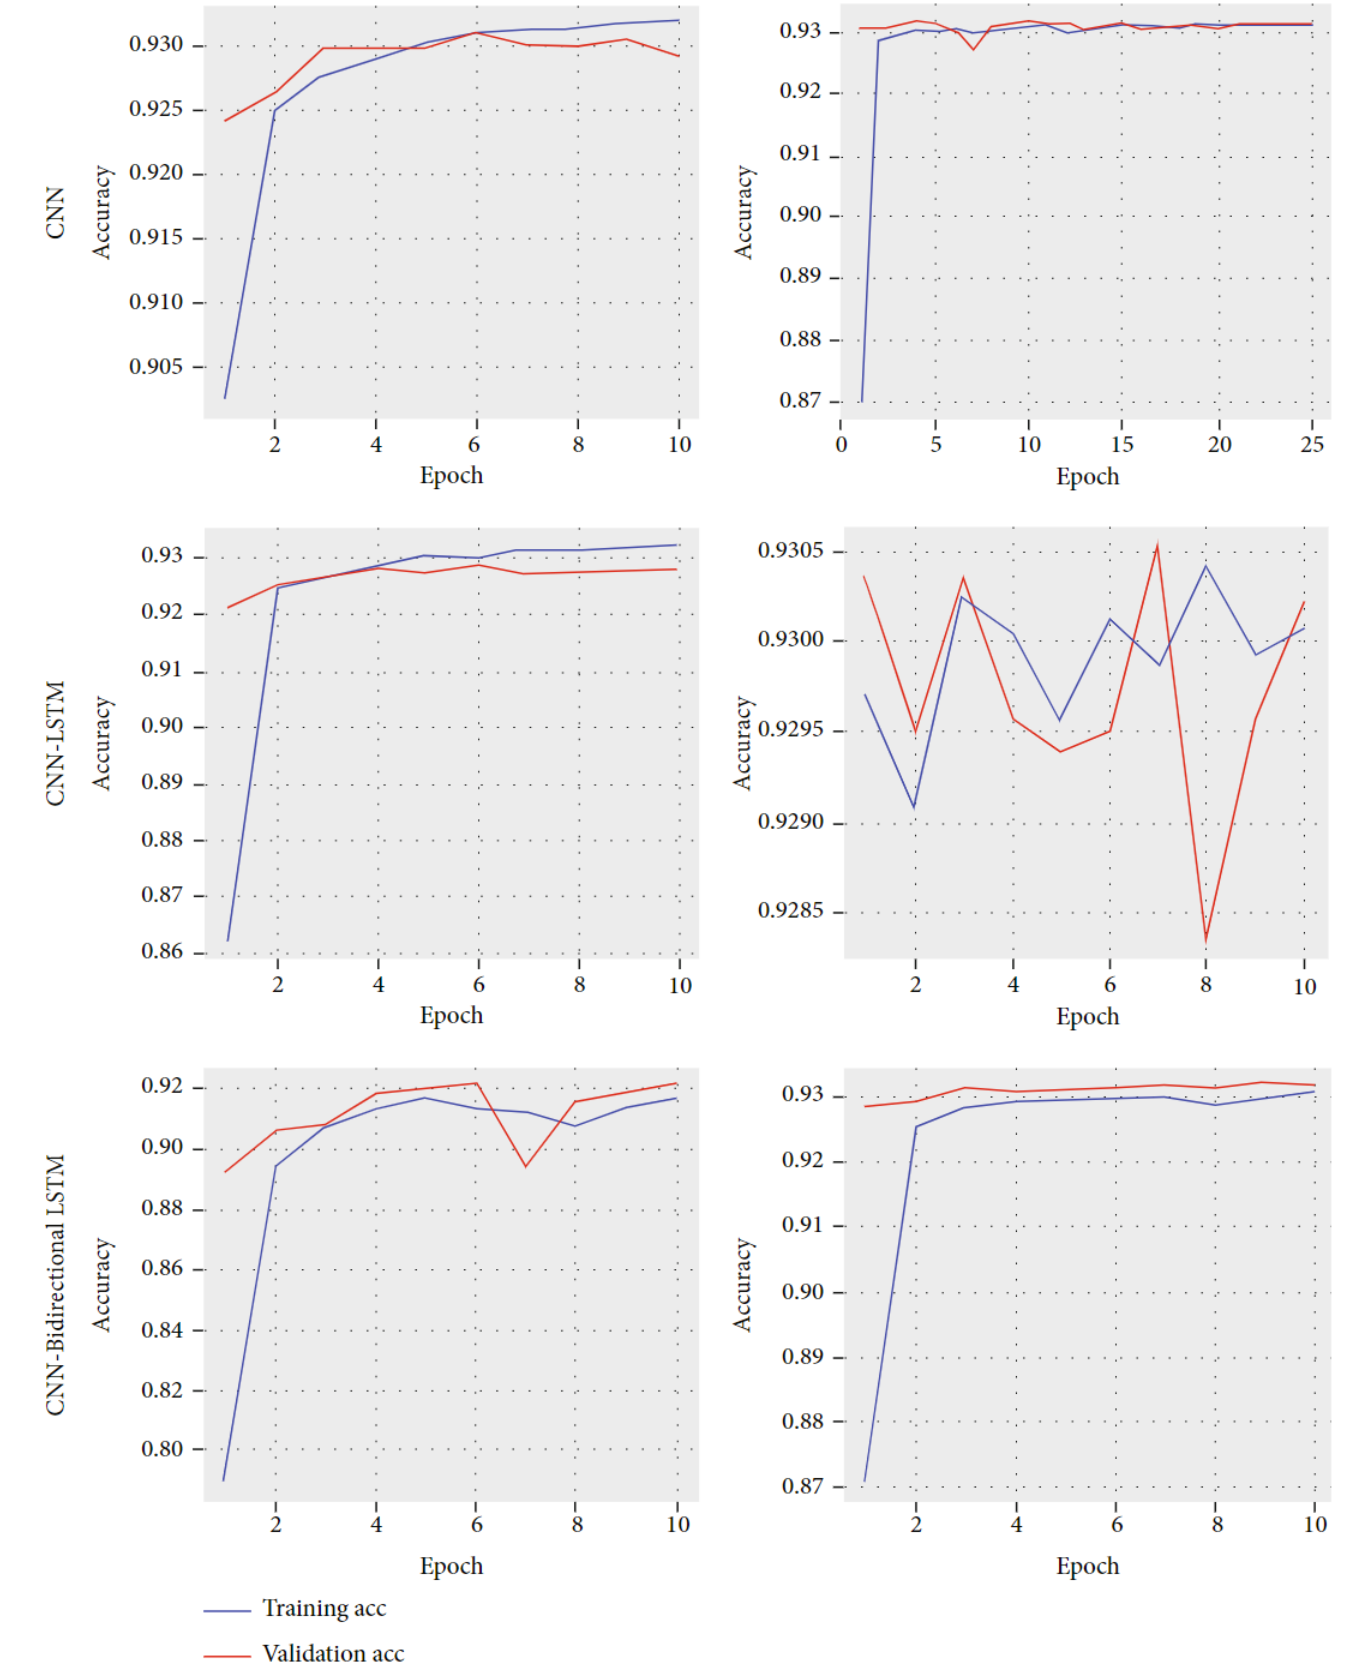
\includegraphics[width=\textwidth]{figures/train_vrs_valid_accuracies.png}
  \caption{Training / Validation accuracies for all six models, borrowed from Gunasekaran, et al. (2020)}
\end{figure*}

\begin{figure*}[t]
\centering
  \caption{Performance Metrics for all Models, borrowed from Gunasekaran, et al. (2020)}
  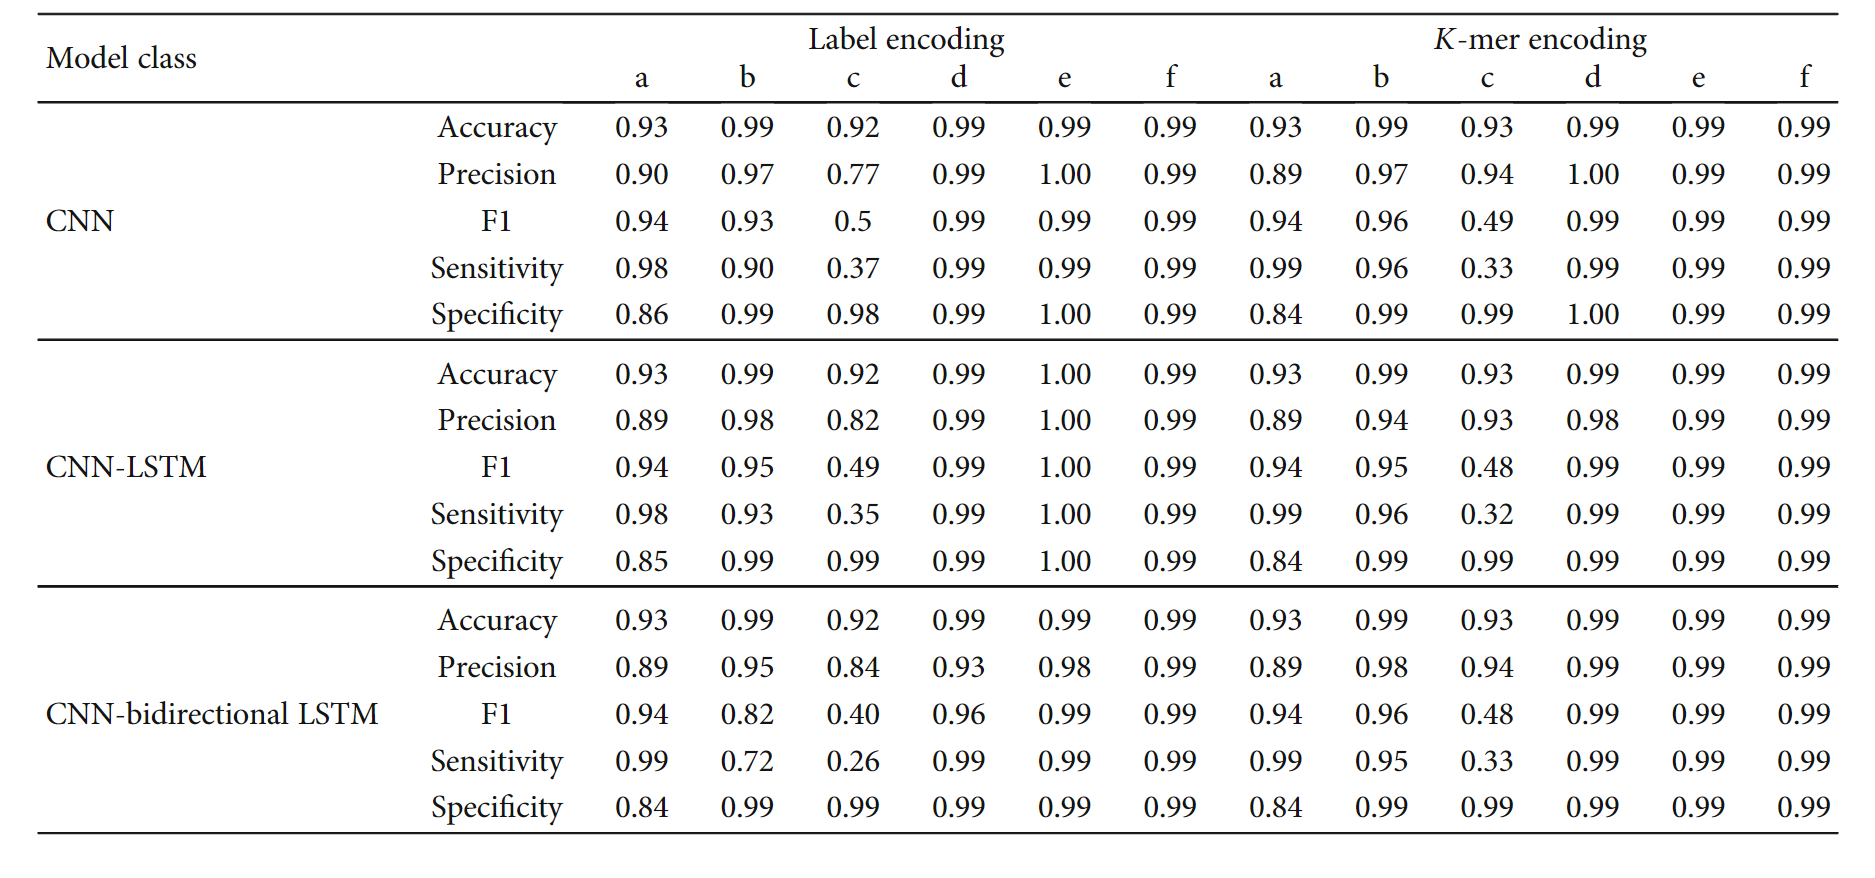
\includegraphics[width=\textwidth]{figures/performance_metrics.png}
\end{figure*}

\end{document}
